\begin{frame}[fragile]{Uso de TabHost y TabWidget en Android}
\textbf{¿Qué son TabHost y TabWidget?}

\begin{itemize}
    \item \textbf{TabHost:} Contenedor principal que gestiona múltiples pestañas (tabs).
    \item \textbf{TabWidget:} Componente visual que muestra las pestañas en la interfaz.
    \item Permiten organizar contenido en diferentes secciones dentro de una misma Activity.
\end{itemize}

\vspace{0.3cm}

\textbf{Estructura básica:}
\begin{itemize}
    \item TabHost contiene:
    \begin{itemize}
        \item Un \textbf{TabWidget} (las pestañas).
        \item Un \textbf{FrameLayout} (contenido de cada tab).
    \end{itemize}
\end{itemize}

\end{frame}


\begin{frame}[fragile]
\frametitle{Demo 12: Pestañas (Tabs)}
\begin{columns}
\column{0.80\linewidth}
Del Repositorio Github:
\begin{itemize}
\item Copiar el archivo \textit{MainActivity\_Demo12.java} (dentro del Folder códigosJAVA) al mismo directorio donde esta el MainActivity.java
\item Copiar el archivo \textit{activity\_main\_demo12.xml} (dentro del Folder Carpeta\_layout) al mismo directorio donde esta el activity\_main.xml
%\item Copiar el archivo \textit{custom\_dialog.xml} (dentro del Folder Carpeta\_layout) al mismo directorio donde esta el activity\_main.xml.
\item Modificar en el archivo \textit{AndroidManifest.xml} la cadena \textit{.MainActivity\_Demo11} por \textit{.MainActivity\_Demo12}.
%\item Ir a la linea 22 de archivo del archivo \textit{MainActivity\_Demo09.java}, poner el cursos en la palabra (en Rojo) \textit{documentfile}, presionar la combinación ALT+ENTER, y seleccionar de la lista desplegable la opcion ``Add dependency on ....''. Esto quitará el error y hara los ajustes necesarios. 
\end{itemize}

%\begin{block}{Demo \#09}
%Un App que permite escribir el contenido de un EditText a un archivo y cargar el contenido de cualquier archivo en el EditText
%\end{block}


\column{0.20\linewidth}

\begin{center}
 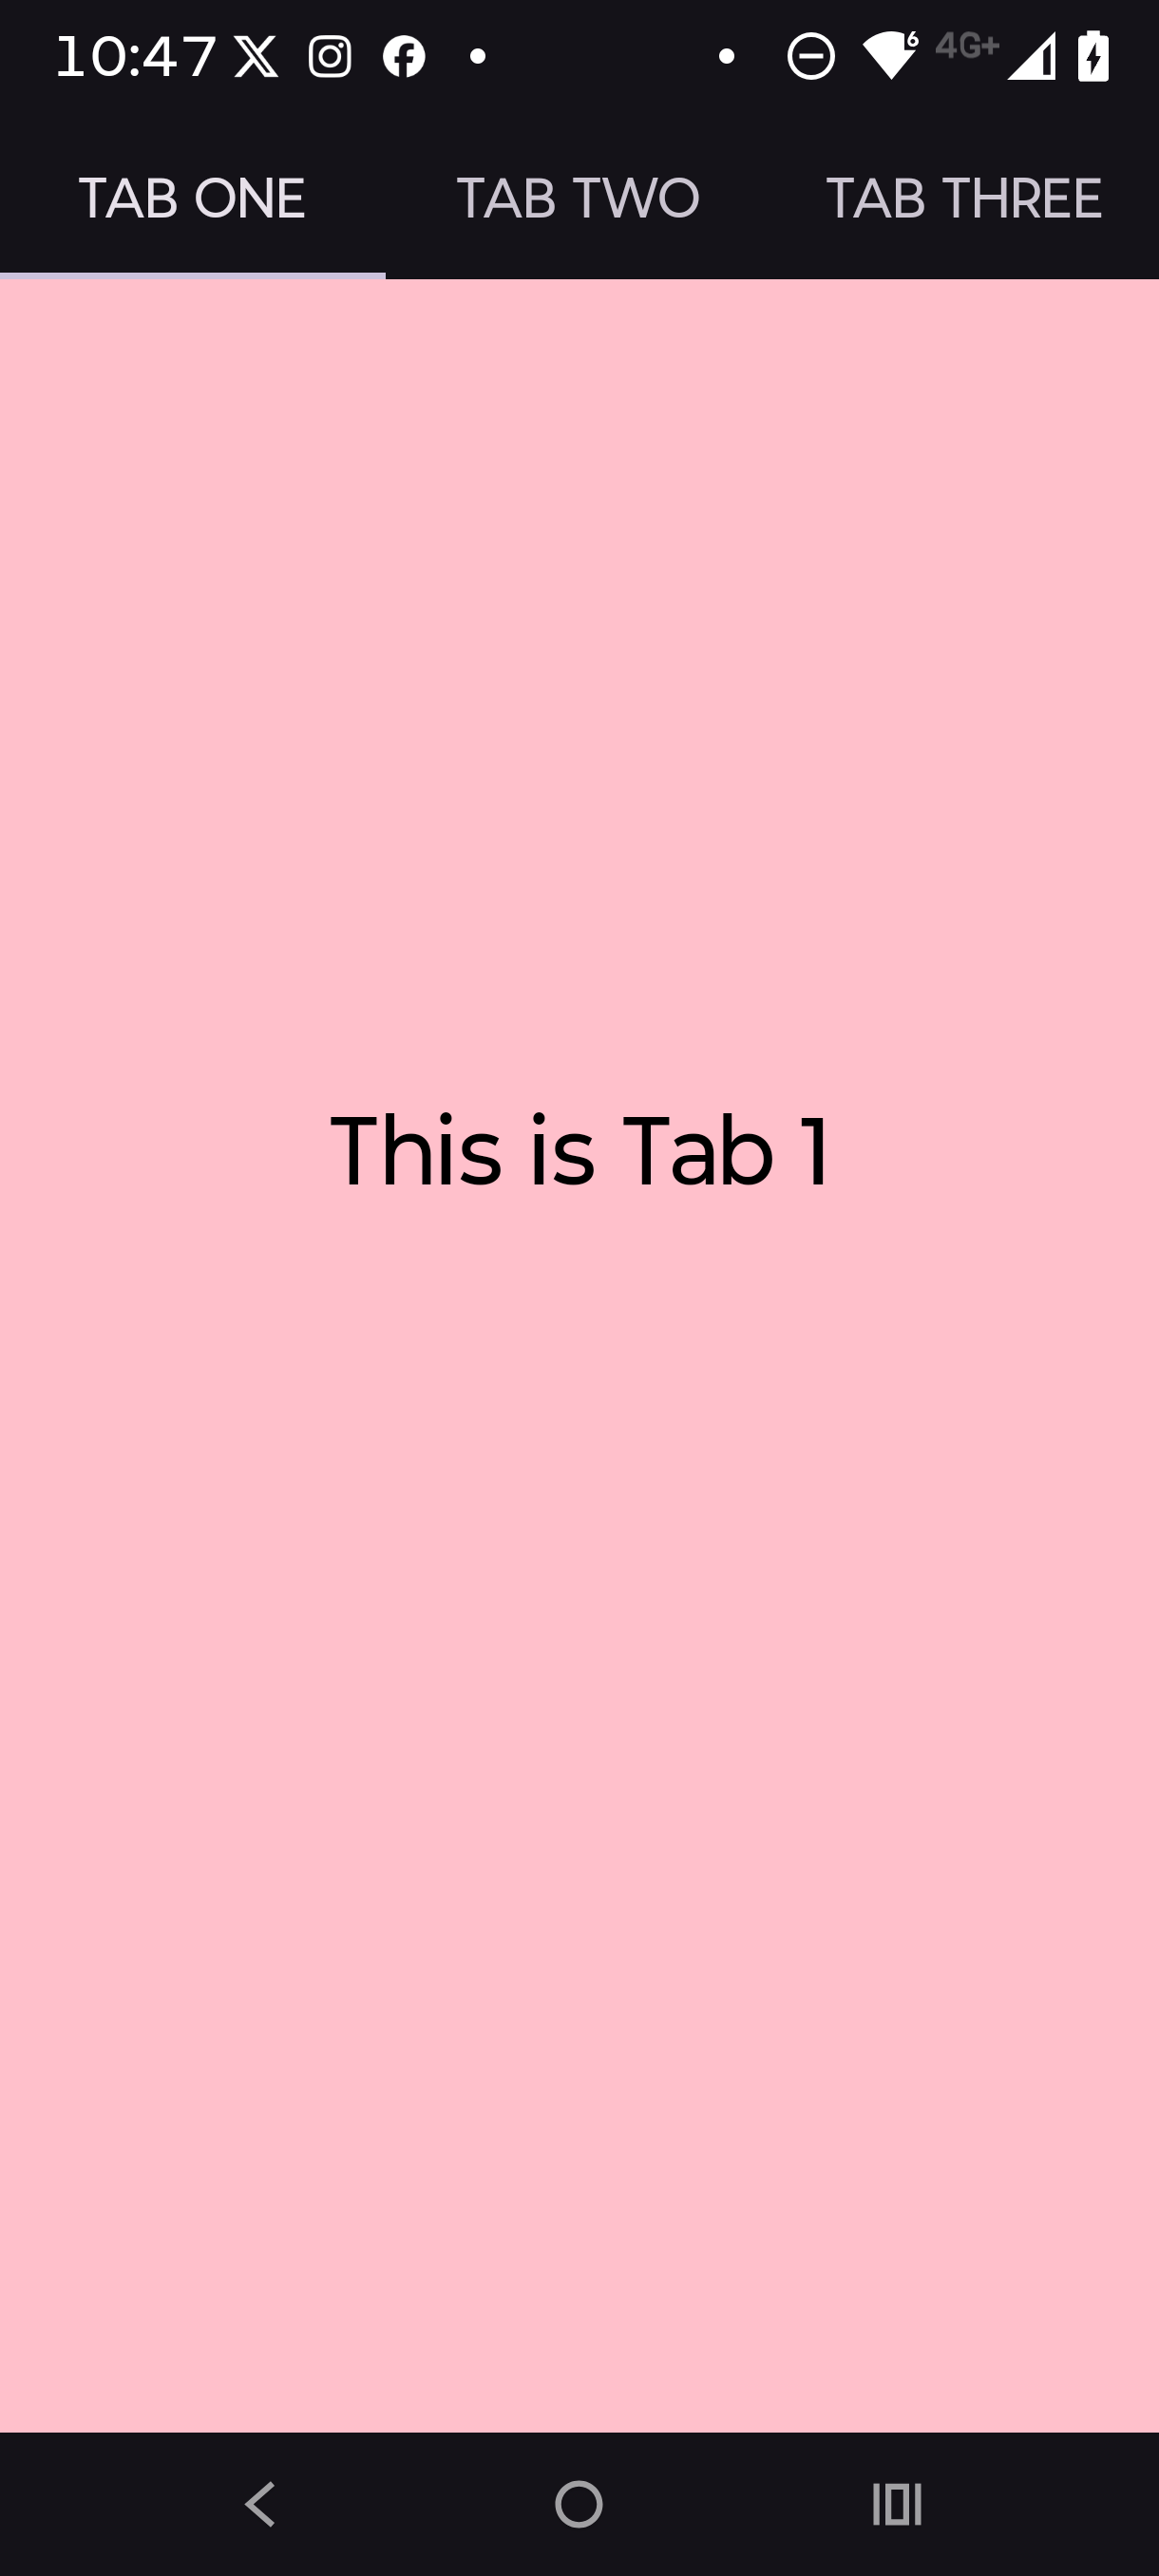
\includegraphics[width=0.98\textwidth]{02_TallerCBTis/figs/Demo12}
\end{center}

\end{columns}

\end{frame}

